
\section{Registro de Cuenta}
El registro de la cuenta del usuario consiste en que el usuario debe de ingresar todos los datos correspondientes a su perfil y seleccionar los roles a los cuales estará asociado, para que se le puedan asignar las acciones a las que podrá acceder.

\subsubsection{Procedimiento}
\begin{enumerate}
	
	\item Presiona el botón \textbf{Crear cuenta} de la pantalla \textbf{Iniciar Sesión}
	
	\begin{figure}[!htbp]			\hypertarget{fig:IniciarSesion}{\hspace{1pt}}
		\begin{center}
			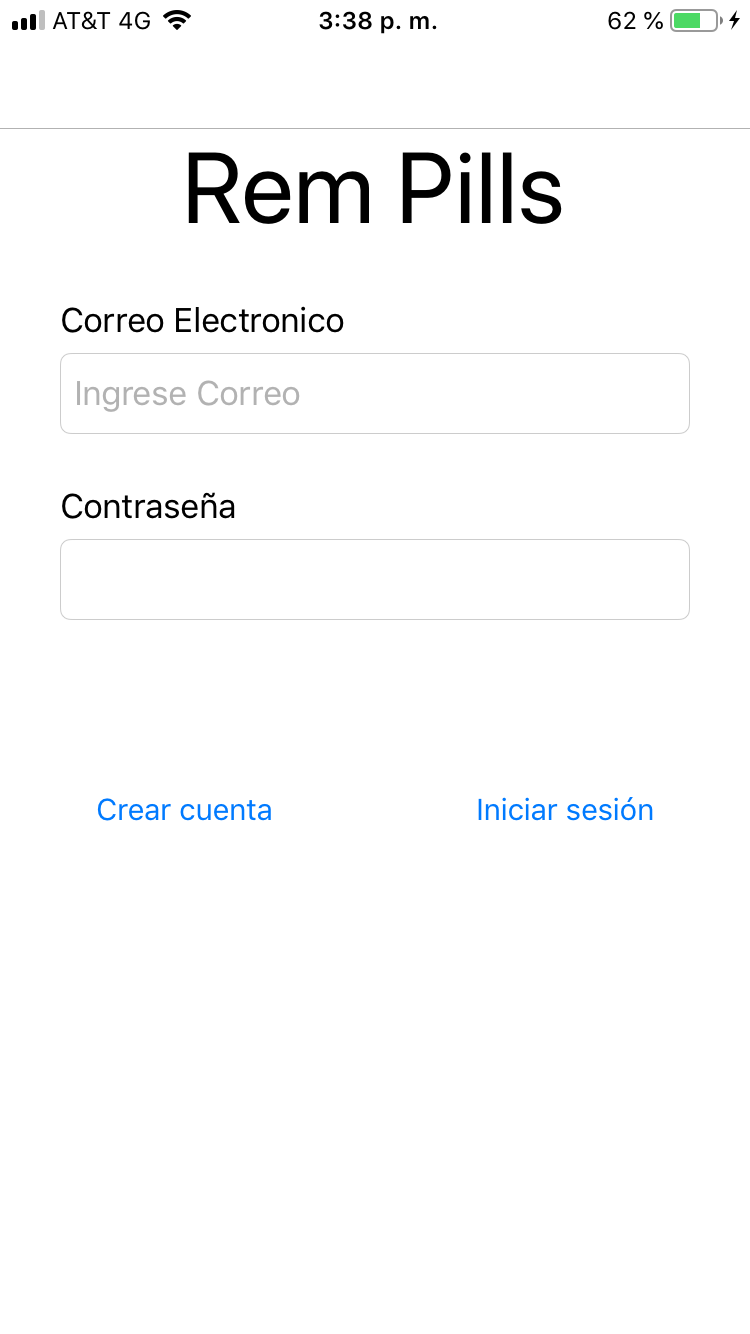
\includegraphics[height=0.4\textheight]{Paciente/RegistrodeCuenta/images/IMG-3180}
			\caption{Iniciar Sesión}
			\label{fig:IniciarSesion}
		\end{center}
	\end{figure}

	\item Se mostrará la pantalla \textbf{Crear Cuenta}
	\newpage
		\begin{figure}[!htbp]			\hypertarget{fig:crearCuenta}{\hspace{1pt}}
		\begin{center}
			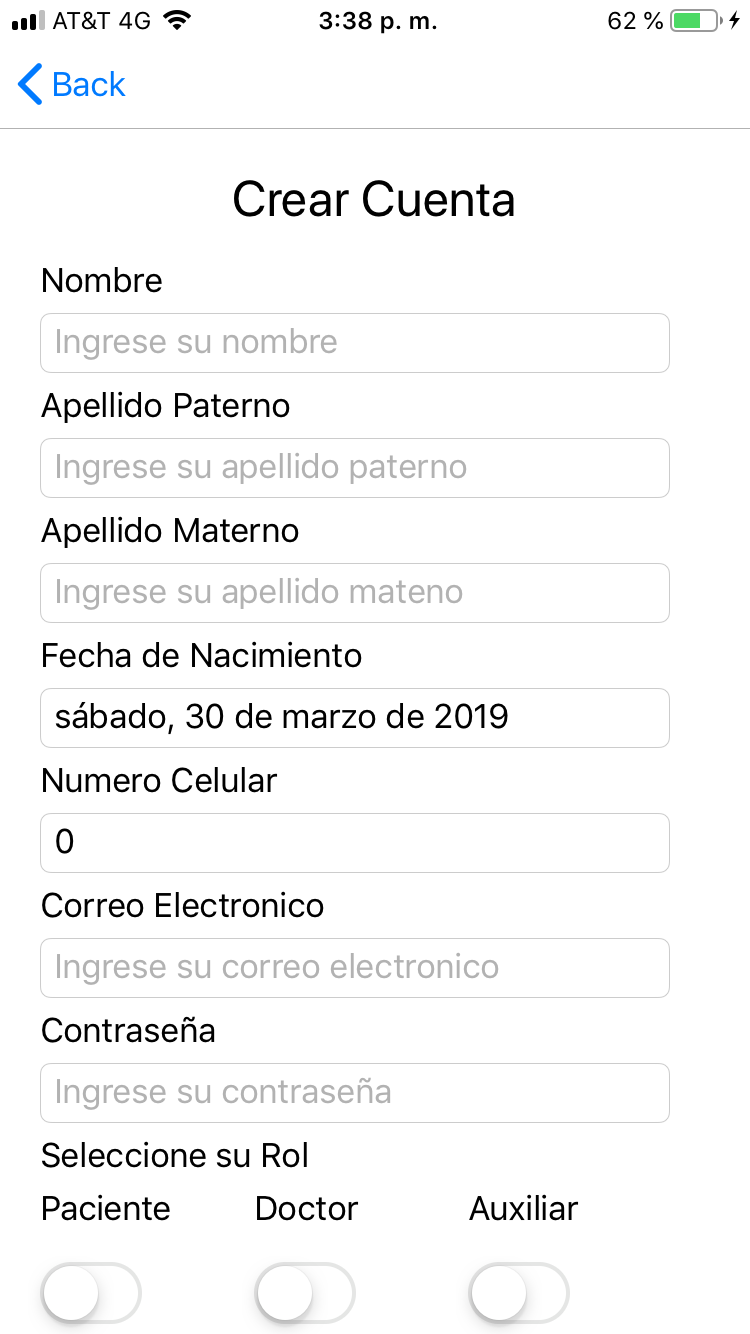
\includegraphics[height=0.4\textheight]{Paciente/RegistrodeCuenta/images/IMG-3181}
			\caption{Crear Cuenta}
			\label{fig:crearCuenta}
		\end{center}
	\end{figure}

	\item Ingresa los datos solicitados por la pantalla \textbf{Crear Cuenta}.
	
	\item Selecciona el rol de Auxiliar.
	
	\item Da clic en el botón Crear Cuenta
	
	\item Se mostrará la pantalla \textbf{Foto de perfil}
	\newpage
	\begin{figure}[!htbp]			
		\hypertarget{fig:fotoPerfil}{\hspace{1pt}}
		\begin{center}
			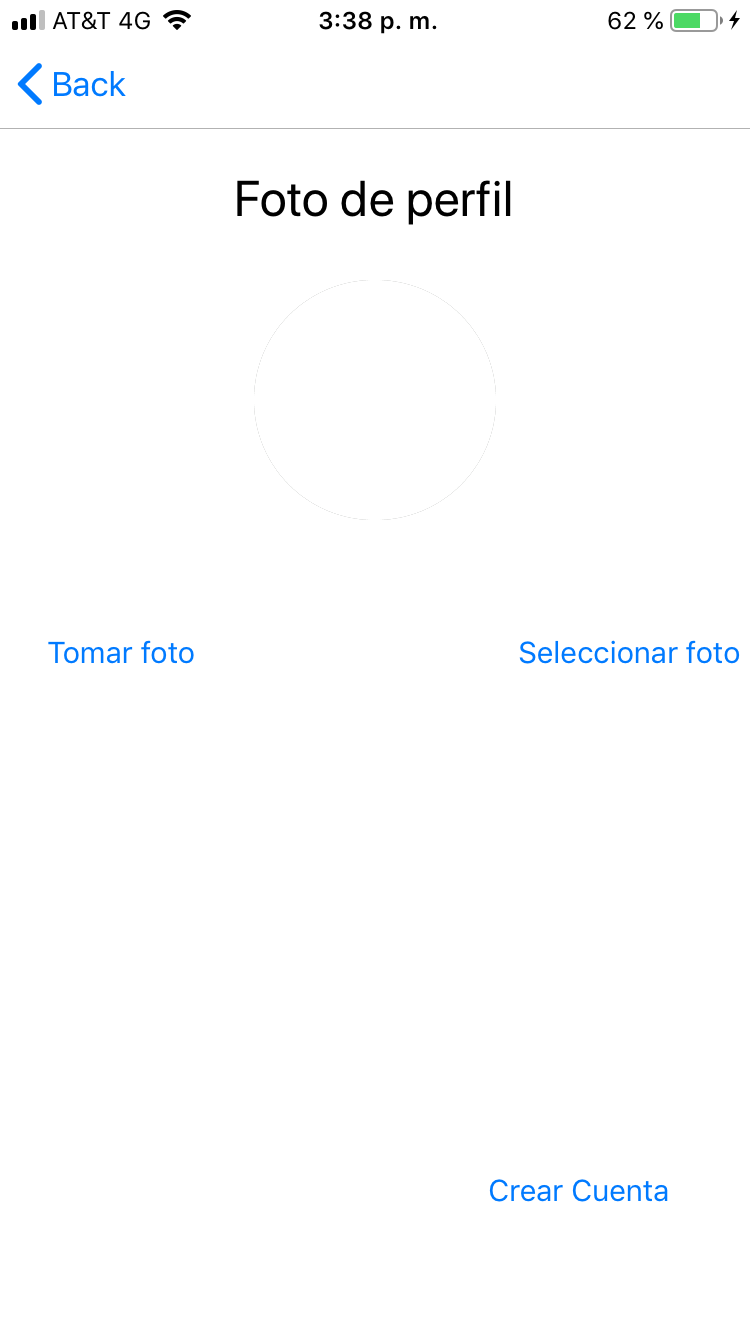
\includegraphics[height=0.4\textheight]{Paciente/RegistrodeCuenta/images/IMG-3182}
			\caption{Foto de Perfil}
			\label{fig:fotoPerfil}
		\end{center}
	\end{figure}

	\item Toma una foto desde tu cámara o selecciona una foto desde tu galería para tu foto de perfil.
	
	\item Da clic en el botón \textbf{Crear Cuenta}

\end{enumerate}

